\subsection{RQ4: Which Oracle Sees Which Fault?}
\label{sec:adequacy}

Our repository has 140 tests: 22 unit, 42 ``conformance'' and 76 integration tests. As committed, 59 of the 76
integration tests fail when run together, because of a hard-coded login limit and a CSRF header that the tests
predate. We lifted both with an external pytest plugin, without changing the application, and then all 138
non-skipped tests of v1 pass (2 are skipped). Coverage is 95\,\% for the PDP, but only 25\,\% for the PEP and 28\,\% for the delegation
workflow. The coverage numbers turned out to predict the mutation results quite well.

\paragraph{Decision logic.} We generated 96 mutants of the v1 PDP. Of these, 13 are equivalent on valid inputs,
3 differ only at the instant a validity bound is reached, and 1 needs inconsistent administrator flags, which
leaves 79. The 3 boundary mutants are not harmless: a frozen-clock oracle that sets a grant's bound equal to the
clock kills all three, and two of them allow a request at the very instant its grant ends.
Figure~\ref{fig:mut}a shows how many each oracle kills. The 11 that escape the L1 oracle all change the database
queries on the cache-miss path, and the L2 cold-cache oracle kills every one of them. Of the 7 that escape our
whole repository suite, 4 are state-level mutants that only E1b detects: they honour assignments that are not yet
valid, delegations held by other subjects, delegations for other objects, and delegations that were never
approved.

\paragraph{Enforcement and cache code.} We then mutated the code we had written for v2: the single PEP gate, the
document-read decision, both revocation handlers, the versioned cache, the post-commit invalidation hooks, and the
middleware that passes the client address to the document route. The same operators as above give 159 mutants of
the final v2; we drop the 2 that mutate the switch used only by the cost ablation, which leaves 157 (the set
differs from earlier versions because the gate and document code changed). The repository suite kills 21 of them
(13.4\,\%) and the 57-check L3 probe kills 116 (73.9\,\%); together they kill 118 (75.2\,\%), and only 2 are
killed by the repository suite alone (Figure~\ref{fig:mut}b). The probe grew with the analysis. A first version
with 11 safety and 6 liveness checks killed 72 of the 158 mutants of an earlier v2; the survivors that could grant
access led to new checks, and the 29-check version killed 105 of those 158. A 38-check version missed a mutant
that drops the address-change term of $\rho$, because no check changed the client address; the checks S24--S25
now do, and kill it. The 39 survivors of the final run are shown in Figure~\ref{fig:mut}c. We inspected each one
by hand:
\begin{itemize}
\item 11 only stop the grant cache from being read or written, so every decision falls back to the database;
\item 7 are equivalent on the attribute domain (for example, no clearance has rank below~1, so comparing with 0, 1
or $-1$ in the classification barrier gives the same result);
\item 5 scale a cache lifetime by $\pm0.1\,\%$ or move a cut-off by 1\,ms;
\item 3 change only decision metadata, such as the measured latency;
\item 3 change the notice sent after a revocation;
\item 2 are masked by a redundant defence: the cache entry's lifetime already ends with the grant, so the expiry
check at read time never fires;
\item 2 make the cache return a malformed value after a Redis error, which the PDP rejects with a server error,
so the request fails closed;
\item 2 change the decision only for a published document with no linked object at all, a state that no route
creates (publishing always links an object, and objects are only deactivated, never removed);
\item 1 bumps the global generation on every bulk write, which only causes extra cache misses.
\end{itemize}
These 36 survivors cannot change a decision, an effect or a record in a state the API can reach. The other three
can. The first makes the document route's risk check strict ($>$ instead of $\geq$), so a request whose score is
exactly $\theta$ is no longer denied there; for a published document the PDP's own $\Px$ still denies it, but for
an unpublished one the workflow rules can then allow it. The probe's risk fixtures reach $\theta$ only on published documents, where the PDP's own check also denies.
The second flips the department test of the owner exemption from the barrier, so an owner whose clearance is
below her own draft's sensitivity can no longer read it; nothing is granted, but access is lost. The third gives
internal calls from the collaboration server that server's address instead of \texttt{unknown}, so the
address-change term can refuse a collaborator's session; again it can only deny. We then ran the bounded
document check E1c (\S\ref{sec:rq5}) against the document survivors. It kills the first two (the first through
97{,}524 R6 violations at $\rho=\theta$, all on unpublished documents, the second through 11{,}016 disagreements
with $\mathcal{M}_{\mathrm{doc}}$) and both unreachable-state mutants (11{,}520 violations of R1--R3 each), and agrees on every world with the three equivalent ones.
Nothing we have kills the third. The lesson is the one the earlier versions taught: a probe checks only the
inputs its fixtures vary, and a bounded check of the same procedure covers the values in between.

\paragraph{Held-out operators.} Because the probe grew while we studied survivors of the operators above, its
score on them may flatter it. We therefore froze the 57-check probe and applied three operators we had not used
while building it, to the same functions: statement deletion, turning a \texttt{raise} into a silent return, and
swapping the first two arguments of a call. This gives 111 mutants; 2 fall inside the ablation switch, which
leaves 109. The probe kills 76 (69.7\,\%), close to its 73.9\,\% on the original operators, and the repository
suite kills 34 (31.2\,\%), every one of which the probe also kills. Of the 33 survivors, 30 cannot change a
decision, an effect or a record: 7 bypass the cache, 6 are equivalent (for example, a flush that the commit at
the end of the request repeats), 6 are masked by a redundant defence (each grant entry is keyed by both the
subject's and the object's counter, so dropping either increment is harmless), 6 only change an error response,
3 change metadata that no rule reads, and 2 change the revocation notice. Three can change a record, and none can
grant access: two drop the audit row written when a delegation or an assignment is revoked (the revocation still
takes effect), and one lets an authorised revoker revoke a delegation that was never approved. The probe counts
the decision and audit rows of access requests, not of administrative changes, so both gaps are again inputs it
does not vary.

\begin{figure*}[t]
\centering
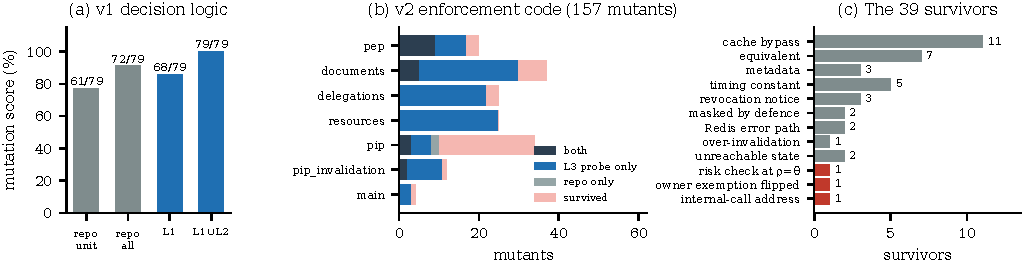
\includegraphics[width=0.92\textwidth]{figs/fig_mut.pdf}
\caption{Mutation analysis. (a) v1 decision logic: share of the 79 non-equivalent PDP mutants killed by each
oracle. (b) v2 enforcement and cache code: mutants per file by the oracle that kills them (repository suite,
L3 probe, both) or surviving. (c) The survivors of (b), by class; grey classes cannot change a decision in a
state the API can reach, red ones can.}
\label{fig:mut}
\end{figure*}

\begin{table}[t]
\caption{Mutation scores per oracle. Top: v1 PDP decision logic (79 non-equivalent mutants). Bottom:
enforcement and cache code of v2, with the original and with held-out operators.}
\label{tab:mut}
\small
\begin{tabular}{@{}lrr@{}}
\toprule
Oracle & killed & score \\
\midrule
Repository unit + conformance suites & 61 / 79 & 77.2\,\% \\
Repository, all 140 tests & 72 / 79 & 91.1\,\% \\
L1 differential oracle (E1) & 68 / 79 & 86.1\,\% \\
L1 $\cup$ L2 (E1, E1b) & 79 / 79 & 100\,\% \\
\midrule
Repository suite on v2 enforcement code & 21 / 157 & 13.4\,\% \\
L3 probe, first version (11 + 6 checks)$^{*}$ & 72 / 158 & 45.6\,\% \\
L3 probe, 29 checks$^{*}$ & 105 / 158 & 66.5\,\% \\
L3 probe, final (34 + 23 checks) & 116 / 157 & 73.9\,\% \\
Repository suite $\cup$ final L3 probe & 118 / 157 & 75.2\,\% \\
Held-out operators: repository suite & 34 / 109 & 31.2\,\% \\
Held-out operators: frozen L3 probe & 76 / 109 & 69.7\,\% \\
\midrule
\multicolumn{3}{@{}p{0.95\columnwidth}@{}}{\footnotesize $^{*}$On an earlier v2 (158 mutants). Of the 39 survivors
of the final run, 36 cannot change a decision, effect or record in a reachable state; E1c kills two of the other
three (Fig.~\ref{fig:mut}c).} \\
\bottomrule
\end{tabular}
\end{table}

\answer{4}{Our repository's tests catch faults in the decision logic (72 of 79 mutants) but hardly any in the
enforcement and cache code (21 of 157). The level oracles catch both: L1 and L2 together kill all 79 decision
mutants, and the L3 probe kills 116 of the 157 enforcement mutants. Of the 39 survivors, three can change a
decision in a reachable state; a bounded check of the document procedure kills two of them. On operators held
out while it was built, the frozen probe scores about the same (76 of 109), and no survivor can grant access.
Each survivor that mattered pointed at an input our fixtures did not vary, not at a fault in v2.}

\subsection{RQ5: Repair, Cost and Comparison}
\label{sec:rq5}

\subsubsection{Repairing \sysname}

\paragraph{Design rules.} The findings suggest six rules.
\textbf{DR1}: put risk denies before every allow rule, or use deny-overrides, and lint for deny-after-permit
redundancy.
\textbf{DR2}: test grants as $a\in G$, keep the scope condition in every allow rule, and let a delegation
actually reach its allow rule.
\textbf{DR3}: make cached grants validity-aware ($\mathit{TTL}=\min(\tau,t_{\mathrm{end}}-t)$) and versioned, and
invalidate \emph{after} the commit, much as Zanzibar uses consistency tokens \cite{pang2019zanzibar}.
\textbf{DR4}: send every protected read through one decision procedure, and let the endpoint, not the client,
choose the action.
\textbf{DR5}: write decisions in their own transaction.
\textbf{DR6}: test each property at the level where it lives.

\paragraph{The repaired chain.} $\mathcal{F}$ moves $\Px$ to just after the administrator rule, adds $\sameDept$ to
$P_4$, puts $P_6$ before $P_5$ (which then denies every employee who holds no grant for the action), and uses
$\sameDiv$. It also makes the owner rule a rule of the chain: $\Po$, with guard $\ow(u,o,a)$, follows $P_3$, and
$\Pc$ exempts it as it exempts $P_2$ and $P_3$ (C3). In v1 this rule was a constant outside the PDP
(\S\ref{sec:system}). Finally, $P_4$ grants read only, whatever else the assignment lists, which removes drift D1
(C4). z3 proves every requirement, R1--R7 and LP, for $\mathcal{F}$ over unbounded domains
(Table~\ref{tab:verdict}). LP holds with the owner exception: an owner needs no assignment to open her own
object.

\paragraph{\sysname v2.} We implemented DR1--DR5 as v2 (15 files, $+$579/$-$289 lines, kept in a separate
history whose first commit is v1). Most of it is straightforward. The cache is not, so Algorithm~\ref{alg:cache} and
Figure~\ref{fig:cache} describe it in detail. Every cached grant is keyed by three generation counters, one global, one per
subject and one per object. A cache fill uses the counters it read \emph{before} querying the database. An
SQLAlchemy \texttt{after\_commit} hook bumps the counters for every ORM or bulk change to a grant, so no endpoint
has to remember to invalidate. Entries also carry the grant's end of validity. Beyond the cache, v2 changes
eight things. One gate serves all file endpoints and decides every request with the PDP, owners included.
Document reads are decided by the PDP on the linked object, with the same request context as the gate, and
every route that lists documents or reads or changes their parts (comments, signatures, delegations shown with
them) applies the same decision, while workflow routes act only within the actor's department. An assignment
grants read only.
Decision and audit rows are written in their own transactions. Revocation requires authority. The PAP refuses to
show built-in rules as inactive. The collaboration server re-checks open sessions every 5\,s. Figure~\ref{fig:v2} shows the
resulting request paths next to those of v1 (Figure~\ref{fig:system}).

Our first version of v2 still had a hole, and we only noticed it while drawing that figure. The design of
\sysname lets an object's owner act on it. The first v2 kept that rule in the gate, confined to the owner's
department and with obligations attached, but still \emph{before} the PDP, and so before $\Px$: a high-risk owner
was allowed where $\mathcal{F}$ denies. DR1 held in the PDP and failed at the gate. None of our probes had a
high-risk owner. Our second version evaluated $\Px$ before the owner rule, in the gate and in the document
procedure, and the probe gained two checks (S22, S23). That closed the hole but kept a second decision procedure
for owners, against DR4, and the document procedure had no request address, so its $\Px$ ignored a change of
address. The current v2 removes both: the owner rule is $\Po$ inside the PDP, the gate and the document procedure
only call the PDP, and both pass the request address to it. Three further checks (S24--S26) cover this, and two
liveness checks (L16, L17) keep it from denying too much.

Another hole was in code we had never run. Our fix for F8 adds a loop to the collaboration server that
re-checks every open session every 5\,s. When we first ran the server, for this paper's final measurements, the
loop re-checked nothing: it looked for the open sessions under a property that the version of the
collaboration library we depend on does not have, so it found none, and a removed collaborator kept her session
(0 of 5 trials closed within 30\,s). After a one-line fix, the server closed the session in 10 of 10 trials,
1.9--4.8\,s after the removal, within the bound of the 5\,s period plus one decision. Our probes had exercised
every request path we had listed in the backend, but not the collaboration server, which is a process of its own.

The list itself was the next weakness. Until then, our route inventory came from reading the code. We then
generated it from the web framework's routing table (\S\ref{sec:l3}), probed what it showed, and swept every
route in scope with subjects who must be refused. This found four more holes, all inherited from v1: comment
resolution and signing decided nothing (F15); the document list decided with a query of its own that showed
every published document of the department, content included, and ignored the classification barrier (F16);
any subject could read any delegation (F17); and a director or division manager of one department could
publish, escalate or remove another department's documents and folders (F18). Each fix makes the route apply
the decision its single-object counterpart applies. Seven safety checks (S28--S34) and five liveness checks
(L19--L23) cover them and the read-only assignments; the first liveness check also showed that comment
resolution had always failed with a server error, which we fixed too.

\begin{figure}[t]
\centering
\begin{tikzpicture}[
  font=\scriptsize, node distance=2mm,
  box/.style={draw, rounded corners=1.5pt, align=center, inner sep=1.5pt, minimum height=5mm},
  pep/.style={box, fill=blue!6, text width=17mm},
  dp/.style={box, fill=green!8, text width=20mm},
  st/.style={box, fill=orange!10, text width=14mm},
  arr/.style={-{Stealth[length=1.5mm]}, semithick}]
  \node[pep] (b1) {\texttt{/access/decide}};
  \node[pep, below=of b1] (b2) {\texttt{/pep/access}, \texttt{/preview}, \texttt{/download}};
  \node[pep, below=of b2] (b3) {\texttt{/documents},\\\texttt{/documents/\{id\}}\\and its parts};
  \node[pep, below=of b3] (b4) {collab.\ WebSocket\\(connect, every 5\,s)};
  \node[dp, right=4mm of b2] (gate) {one gate: PDP for every request, owners included; action from endpoint; obligations};
  \node[dp, right=4mm of b3, yshift=-5mm] (doc) {document read: $\Px$ with request address; published $\to$ PDP; draft $\to$ $\Pc$ barrier};
  \node[dp, text width=11mm, right=4mm of gate] (pdp) {PDP\\$=\mathcal{F}$};
  \node[st, right=4mm of pdp, yshift=7mm] (cache) {versioned grant cache};
  \node[st, below=4mm of cache] (pg) {PostgreSQL};
  \node[st, below=4mm of pg] (log) {ledger (own transaction)};
  \draw[arr] (b1.east) -| (pdp.north);
  \draw[arr] (b2) -- (gate); \draw[arr] (gate) -- (pdp);
  \draw[arr] (b3.east) -- (doc.west); \draw[arr] (b4.east) -- (doc.west);
  \draw[arr] (doc.east) -| (pdp.south);
  \draw[arr] (pdp.east) -- (cache.west); \draw[arr] ([xshift=-2mm]cache.south) -- node[left]{miss} ([xshift=-2mm]pg.north);
  \draw[arr, dotted] ([xshift=2mm]pg.north) -- node[right]{bump} ([xshift=2mm]cache.south);
  \draw[arr, dashed] (pdp.south east) -- (log.west);
\end{tikzpicture}
\caption{\sysname~v2: every protected read passes $\Px$ first and is then decided by the PDP (which contains the
owner rule $\Po$) or, for unpublished documents, by the clearance barrier of $\Pc$ followed by the document
rules. Decisions are recorded in their own transaction, and committed grant changes bump the cache
generations.}
\label{fig:v2}
\end{figure}

\begin{algorithm}[t]
\caption{Versioned, validity-aware grant cache (v2)}
\label{alg:cache}
\SetKwFunction{Get}{Lookup}\SetKwFunction{Fill}{Fill}\SetKwFunction{Bump}{OnCommit}
\SetKwProg{Fn}{function}{:}{}
\Fn{\Get{$u,o,g$}}{
  $\vec{n}\gets(\mathit{gen}_\ast,\mathit{gen}_u,\mathit{gen}_o)$ \tcp*{one atomic read}
  remember $\vec{n}$ for this request\;
  $e\gets\mathit{cache}[g,u,o,\vec{n}]$\;
  \lIf{$e\neq\bot\wedge \mathit{now}<e.\mathit{exp}$}{\Return $e.\mathit{actions}$}
  \Return miss\;
}
\Fn{\Fill{$u,o,g,B,t_{\mathrm{end}}$}}{
  $\vec{n}\gets$ the generations remembered \emph{before} the database read\;
  $\mathit{ttl}\gets\min(\tau_g,\,t_{\mathrm{end}}-\mathit{now})$\;
  \lIf{$\mathit{ttl}>0$}{$\mathit{cache}[g,u,o,\vec{n}]\gets(B,t_{\mathrm{end}})$ with lifetime $\mathit{ttl}$}
}
\Fn{\Bump{$\mathit{tx}$}}{
  \ForEach{grant row $(u,o)$ inserted, updated or deleted in $\mathit{tx}$}{increment $\mathit{gen}_u$, $\mathit{gen}_o$}
  \lIf{$\mathit{tx}$ ran a bulk statement on a grant table}{increment $\mathit{gen}_\ast$}
}
\end{algorithm}

\begin{figure}[t]
\centering
\begin{tikzpicture}[font=\scriptsize, >={Stealth[length=1.4mm]}]
  \draw[->] (0,0) -- (6.9,0) node[right]{$t$};
  \node[anchor=east] at (0,0.8) {revoke};
  \node[anchor=east] at (0,-0.8) {decision};
  \draw[thick, blue!60] (0.2,0.8) -- (3.8,0.8) node[midway, above]{revoking transaction};
  \draw[fill=blue!60] (3.8,0.8) circle (1.4pt) node[below=1pt]{commit};
  \draw[fill=red!70] (5.0,0.8) circle (1.4pt) node[above=1pt]{$\mathit{gen}_u\gets k{+}1$};
  \draw[thick, teal] (1.4,-0.8) -- (6.3,-0.8);
  \draw[fill=teal] (1.4,-0.8) circle (1.4pt) node[below=1pt]{read gens: $k$};
  \draw[fill=teal] (3.1,-0.8) circle (1.4pt) node[below=1pt]{DB read (old state)};
  \draw[fill=teal] (6.3,-0.8) circle (1.4pt) node[below=1pt]{fill under $k$};
  \draw[dashed, gray] (5.0,0.65) -- (5.0,-1.15);
  \node[align=center, text width=64mm] at (3.4,-1.6) {every lookup after the bump uses generation $k{+}1$, so the stale fill is never served};
\end{tikzpicture}
\caption{Why the v2 cache closes the race: a fill that read the database before the commit is stored under the
old generation, which no lookup after the commit can reach.}
\label{fig:cache}
\end{figure}

The cache earns a small theorem of its own, in the safe direction: whatever it reports as granted was granted
recently.

\begin{proposition}[Freshness of the v2 cache]\label{prop:fresh}
Assume (i) every committed transaction that changes a grant of $(u,o)$ increments $\mathit{gen}_u$ and
$\mathit{gen}_o$, or $\mathit{gen}_\ast$ for a bulk statement, within $\epsilon_b$ of its commit; (ii)
\textsc{Fill} stores the action set read from committed state under generations observed before that read;
(iii) no entry is served at or after its grant's end of validity; (iv) \textsc{Lookup} reads the generation vector
and the entry in one atomic step, which is its linearization point $t$ in the sense of
\cite{herlihy1990linearizability}; and (v) counters never decrease. If \textsc{Lookup} at time $t$ returns $B$ for
$(u,o,g)$, then $B=G^g_{t'}(u,o)$ for some $t'\in[t-\epsilon_b,t]$, unless the grant became valid at a future
start time without any commit, which can only make the cache deny.
\end{proposition}
\begin{proof}
Let the entry have been filled from a read of $\sigma_{t_r}$ under generations $\vec{n}$ observed at
$t_n\le t_r$; so $B=G^g_{t_r}(u,o)$, possibly up to grants that ended after $t_r$, which (iii) excludes. If
$t_r\ge t-\epsilon_b$, take $t'=t_r$. Otherwise suppose some commit at $t_c\in(t_r,t-\epsilon_b]$ changed a grant
of $(u,o)$. By (i) a generation in $\vec{n}$ was incremented by $t_c+\epsilon_b\le t$. Counters only grow, so the
lookup at $t$ read a vector different from $\vec{n}$ and could not have found the entry, a contradiction. Hence
no grant of $(u,o)$ changed by commit in $(t_r,t-\epsilon_b]$, and with (iii) $B=G^g_{t-\epsilon_b}(u,o)$.
\end{proof}

In the code, (i) holds with $\epsilon_b$ the time between the database commit and the Redis increments in the
same process; (ii) holds because the generations read at the miss are kept in the request context and reused
by the fill; (iii) is enforced twice, by the entry's lifetime and by an explicit check; (iv) holds because one Redis
script reads the counters and the entry; and (v) holds because counters and entries live in the same Redis, so a
restart or flush removes both. Assumption (i) is conditional: if the increments fail, for instance because Redis
is unreachable, the hook logs the failure and only Theorem~\ref{thm:stale} applies, bounding the window by
$\tau_g$. A crash between commit and increment has the same effect.

We measured both cases on the running server. Under a load of 16 clients sending file requests, we created and
revoked an assignment 200 times, with one and with two server workers, and timed the hook in the server process.
Over the 400 commits of each setting, $\epsilon_b$ had a median of 0.79 and 0.70\,ms, a 99th percentile of 3.7 and
3.0\,ms, and a maximum of 4.8 and 4.4\,ms; in all 400 revocations the counters had moved before the revocation's
response was sent, and the next request was denied. We then made the hook's connection to Redis fail during the
revocation, while the cache itself stayed up, in five trials each with a refused connection and with a timeout.
In all ten, the increment was lost and the revoked grant kept working for 118--120\,s, that is, until the
cached entry's lifetime of $\tau_{\mathrm{asg}}=120$\,s ran out, as Theorem~\ref{thm:stale} predicts. The timeout
also showed a cost we had not expected: the hook uses a synchronous Redis client, so the 2\,s timeout blocks the
server's event loop, and an unrelated request sent meanwhile took 1.8\,s instead of 12--21\,ms.

Both grant kinds use the same counters, so a commit on either invalidates both entries of the pair, and the two
grant sets of a decision come from states at most $\epsilon_b$ apart. That is still a view, not a snapshot, but
$\mathcal{F}$ satisfies the premise of Proposition~\ref{prop:witness}. Hence every v2 allow is justified by a
committed state at most $\epsilon_b$ old, provided the attributes of $u$ and $o$ (read from the database at decision
time) did not change in that interval: v2 is L2$^+_{\epsilon_b}$ under this proviso, and with the gate it meets the
premise of Theorem~\ref{thm:compose} with $\Delta=\epsilon_b$.

\smallskip\noindent\fbox{\parbox{\dimexpr\columnwidth-2\fboxsep-2\fboxrule\relax}{\small
\textbf{What the end-to-end guarantee for v2 assumes.} Theorem~\ref{thm:compose} gives, for v2, that every effect is
justified by a committed state at most $\epsilon_b+d$ old, and every decision is recorded, if:
\begin{enumerate}[leftmargin=*,nosep]
\item runs are well-formed (W1--W3, Def.~\ref{def:runs}), and an effect follows its decision within $d$;
\item every committed grant change increments its counters within $\epsilon_b$ (measured: at most 4.8\,ms under load);
\item the subject's and object's attributes do not change between the cache fill and the decision (they are read
from PostgreSQL at each decision, at the default isolation level, \texttt{READ COMMITTED});
\item the trusted base of \S\ref{sec:threat} (database, cache, administrators, deployed code) is not compromised;
\item every path to a protected object is in the L3 inventory and its checks pass.
\end{enumerate}
If (2) fails because Redis is unreachable at commit, only the TTL bound $\Delta=\tau$ of Theorem~\ref{thm:stale}
holds (measured: 120\,s for assignments). The guarantee is never one of current-state authorization: an effect
may follow a revocation by up to $\Delta+d$.}}

\paragraph{Does it work?} The v2 PDP equals $\mathcal{F}$ on all 737{,}280 worlds (the 368{,}640 of v1, once
with and once without ownership), violates none of the requirements, LP included (Figure~\ref{fig:l1}a), and
still satisfies criterion G (96 occurrences; the self-test still flags all ten seeded violations). Its observation vector gains two atoms, $[\mathsf{own}(o)=u]$ and $[a=\mathit{download}]$; with them, the
coverage query finds 4{,}320 satisfiable vectors, all realised by the world space, so Theorem~\ref{thm:complete}
applies to v2 as well. With a cold cache, its queries agree with $\Gasg_t$ and $\Gdel_t$ on all 420 lifecycle
worlds, as v1's do. All 57 checks of the L3 probe pass on v2, while v1 fails 31 of the 34 safety checks
(Figure~\ref{fig:l3}), and denials leave 20 of 20 rows on every endpoint. The version of v2 before this paper's last
round of fixes fails all seven new safety checks (S28--S34) and two liveness checks (L19, with a server error,
and L23, because S33 had already published its document), which is how we confirmed that the checks see the holes
they were written for.

The document procedure is not the PDP for unpublished documents, so we gave it an L1 check of its own. We
transcribed it as a reference $\mathcal{M}_{\mathrm{doc}}$ and drove the real procedure, with only its data
sources stubbed as in E1, over 604{,}800 worlds: every role, division and department relation, workflow status,
clearance and sensitivity, ownership, collaboration, linked object (none, active, deleted), grant on that object,
and risk. We checked agreement with $\mathcal{M}_{\mathrm{doc}}$, R1, R2, R3 and R6 (for documents, R3 also accepts
a collaboration invitation on an unpublished document, the guide's mechanism for co-editing drafts), and that a
published document is decided as $\mathcal{F}$ decides its object. The check found a third hole in v2. Deleting a
published document's object (an ordinary soft delete through the API) left the document published, and its reads
fell through to the workflow rules: any employee of the department could read it without a grant (R3), a subject
who had moved could read it with an old assignment (R1), and an owner who had moved escaped the clearance barrier
(R2). The three requirements failed in 384, 1{,}344 and 480 worlds, and 2{,}253 worlds with a deleted object were
decided differently from $\mathcal{F}$. (R3 also failed in 216 worlds of a published document with no object at
all, which the API cannot produce.) The current v2 lets the linked object decide through the PDP whether or not it is
active, refuses a published document without one, and confines the owner's exemption from the barrier to her
department; the check then reports no violation, and the probe has a check for it (S27). All staleness windows shrink to the
resolution of the harness: 0.03--0.05\,s after delegation revocation, 0.02--0.14\,s after expiry, 0.02\,s with the
injected race, and no stale allow in 200 two-worker races (Figure~\ref{fig:l2}c; upper 95\,\% bound 1.9\,\%) or,
on the final v2, in 600 one-worker races (0.6\,\%); the cache and revocation code has not changed since these staleness runs. Of our 140 tests, on v2
137 pass, 2 are skipped (as on v1) and 1 fails. The one that fails asserts that $P_7$, not $P_5$, denies a request
that both rules deny; in $\mathcal{F}$, $P_5$ denies every employee who holds no grant for the action, so it
decides first.

\subsubsection{Cost}

We measured v1 and the final v2 with 16 closed-loop clients on one server worker, three interleaved runs per
version, and 3{,}000 requests per workload and run (Figure~\ref{fig:cost}). On this machine, runs of the same
version differed by up to 42\,\% in their median, so we report a difference only where every run of one version
lies on the same side of every run of the other. Three differences pass that test. Denied file requests, which v2 records in their own transaction, are
32\,\% slower (median 104 to 136\,ms); document reads, which now pay for a full PDP decision and an unindexed
lookup of the linked object, are 47\,\% slower (110 to 162\,ms); and assignment creation is 35\,\% faster (169 to
110\,ms), probably because one counter increment replaces two scans of the cache's key space. For
decisions and allowed file requests, the pooled medians of v2 are 2--9\,\% higher, but the runs overlap, so we
cannot tell them apart from the noise. The 99th percentile of document reads rises from 224 to 326\,ms, and their
throughput falls by 34\,\%; no request failed with a server error in either version. The revocation race,
repeated within these runs, re-admitted a revoked grant in 315 of 600 trials on v1 (52.5\,\%; 95\,\% Wilson
interval 48.5--56.5\,\%) and in none of 600 on v2 (upper bound 0.6\,\%). An earlier measurement with two runs per
version, on a quieter machine and before the last changes to the gate and the document route, gave higher ratios
for decisions (16--25\,\%) and documents (69\,\%); we do not know how much of that gap is the code and how much the
machine. We also ran two workers on an earlier v2. There, medians of the \emph{same} version differed by up to
67\,\% between runs; we suspect an uneven split of the client connections between the two workers, did not verify
it, and draw no conclusion from those runs. Where the cost matters, the obvious next steps are an index on the
document link and batching the decision log; we have not done either.

\begin{figure}[t]
\centering
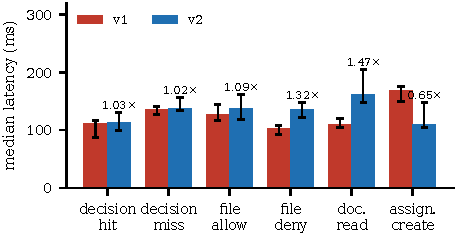
\includegraphics[width=\columnwidth]{figs/fig_cost.pdf}
\caption{Median latency of v1 and the final v2 on one server worker, 16 clients, three runs per version
($n=9{,}000$ per bar). Error bars span the three per-run medians; labels give the ratio v2/v1 of the pooled
medians. Only denied file requests, document reads and assignment creation differ by more than the spread between
runs.}
\label{fig:cost}
\end{figure}

\subsubsection{\chain in Cedar}

A first-applicable chain compiles exactly into Cedar's forbid-overrides semantics. Rule $i$ becomes a
\texttt{permit} when $e_i=\allowv$ and a \texttt{forbid} when $e_i=\denyv$, with the condition
\[
\gamma_i\wedge\textstyle\bigwedge_{j<i,\;e_j\neq e_i}\neg\gamma_j .
\]
A permit fires only if no earlier deny guard holds, and a forbid only if no earlier allow guard holds, so the
first applicable rule decides and no forbid can override it. Cedar's actions are fixed by its schema, so grant
membership expands per action. The compiled policies for $\mathcal{M}$ (36) and $\mathcal{F}$ (40) pass Cedar's
validator, and Cedar's authorizer agrees with our reference on every request: 368{,}640 for $\mathcal{M}$, and
737{,}280 for $\mathcal{F}$, whose owner rule doubles the request space (the requester owns the object or not).
The translation also makes F1 easy to see: in $\mathcal{M}$, the $\Px$ forbid is guarded by the negation of every
allow scope, and deleting it changes nothing. A hand-written 12-policy version of $\mathcal{F}$, with plain
\texttt{forbid} rules for $\Px$, $P_1$ and $\Pc$ and the owner exemption as an \texttt{unless} clause, agrees on
all 737{,}280 requests as well. Under forbid-overrides, DR1 holds by construction.

\subsubsection{\sysname Among Other Authorization Systems}
\label{sec:compare}

We wanted to know whether what we found is specific to our code, and how our design choices compare. We
therefore applied parts of the method, without modifying the systems, to three independent ones. This is a
preliminary transfer: we ran sampled L1 checks, targeted L2 experiments and a few L3 probes, but established
neither criterion G nor coverage nor a route inventory for their code. The systems are:
\begin{itemize}
\item OpenFGA 1.22.1 \cite{openfga}, an open implementation of Zanzibar's relationship model, run from its
release binary;
\item Cedar's TinyTodo sample application \cite{cedarexamples}, built on a verified authorizer;
\item the Backstage RBAC plugin 8.1.6 \cite{backstagerbac}, which keeps policies in a database and takes groups
from a software catalog.
\end{itemize} Zanzibar
itself is not available to run, so we compare with it from its paper \cite{pang2019zanzibar}.
Table~\ref{tab:compare} puts the six side by side; every cell is either measured by us, cited, or marked as not
evaluated.

\begin{table*}[t]
\caption{\sysname compared with other authorization systems. M: measured by us on an unmodified system; C: from
the cited source; n.e.: not evaluated. Bold marks a failure found by our method.}
\label{tab:compare}
\footnotesize
\begin{tabularx}{\textwidth}{@{}l@{\;\;}X@{\;\;}X@{\;\;}X@{\;\;}X@{\;\;}X@{\;\;}X@{}}
\toprule
 & \sysname v1 (M) & \sysname v2 (M) & Zanzibar \cite{pang2019zanzibar} (C) & OpenFGA 1.22.1 (M) & Cedar, TinyTodo (M) & Backstage RBAC 8.1.6 (M) \\
\midrule
Policy model & ABAC rule chain over attributes and grants (\chain) & repaired chain $\mathcal{F}$ & relation tuples; namespace configurations with userset rewrites & Zanzibar-style relationship model & \texttt{permit}/\texttt{forbid} policies over entities \cite{cutler2024cedar} & roles and permission policies in a database; conditional decisions \cite{backstagerbac} \\
Combination & first-applicable & first-applicable; compiles exactly to forbid-overrides & union, intersection, exclusion of usersets & as Zanzibar & forbid overrides permit; default deny & documented precedence rules \\
Assurance & pen-and-paper proofs (one theorem false) & z3 proofs of R1--R7 and LP & n.e. & n.e. & authorizer proved in Lean, differentially tested \cite{cutler2024cedar,disselkoen2024vgd} & n.e. \\
State freshness & TTL cache (60\,s, 120\,s); invalidation before commit, assignments only & versioned keys; bump after commit; validity clamp & snapshot reads at zookie timestamps (``new enemy'') & optional check cache with TTL; \texttt{HIGHER\_CONSISTENCY} bypasses it & state read on each request; policy file reloaded & policies and catalog read per decision; optional group claims in tokens \\
L1 (rule) & \textbf{risk rule inert; read delegation unlocks writes}; PDP $=\mathcal{M}$ on 368{,}640 worlds & PDP $=\mathcal{F}$; R1--R7 and LP hold & n.e. & 5{,}120/5{,}120 checks over 512 tuple states & 0/200 mismatches & 81/81 configurations as documented \\
L2 (state): revocation & \textbf{$\tau-\delta$ (up to 60\,s); race re-admits 98/200} & $\le$0.14\,s (harness resolution); 0/200 & n.e. & 2\,ms; with check cache \textbf{$\tau-\delta$} (10.0 / 5.0\,s), also with the cache controller & next request & next decision; \textbf{token claims until reissue} (default up to 1\,h \cite{backstageauth}) \\
L2 (state): policy & PAP status ignored by the PDP & built-in rules cannot be deactivated & n.e. & n.e. & reload in 0.12--0.90\,s; \textbf{invalid file: new \texttt{forbid} never enforced} (20/20) & per decision \\
L3 (enforcement) & \textbf{five decision procedures; denials lost; routes that decide nothing} & one gate and one document procedure; 57/57 checks & clients call \texttt{Check} & PDP only (no PEP) & 8/8 endpoints mediated; \textbf{principal client-asserted} (demo) & conditional decisions enforced by each plugin \\
\bottomrule
\end{tabularx}
\end{table*}

\paragraph{The rule level agrees wherever we sampled it.} All three external systems agreed with a reference at L1 on
every case we generated, which reassured us that the method does not simply find problems everywhere. This is
sampled agreement, not the complete check of \S\ref{sec:l1}: we did not establish criterion G or coverage for
their code. OpenFGA's \texttt{Check} agreed with a reference
evaluation of a model with group usersets, inheritance and an exclusion on all 5{,}120 checks over 512 tuple
states. TinyTodo's list query, computed by partial evaluation, agreed with per-list authorization in 200 of 200
checks on random states. Backstage's decisions matched its documented precedence rules in all 81 policy
configurations. The rule-level failures of \sysname v1 are failures of our chain, not of the idea of a rule
chain: the same chain compiled to Cedar inherits them, and $\mathcal{F}$ removes them in both.

\paragraph{The state level is where systems differ.} Where state is read on every request, it is fresh. The
failures appear wherever a decision consults a \emph{copy} of authorization state whose lifetime is not tied to
its source, which is the premise of Theorem~\ref{thm:stale}. OpenFGA shows the theorem in its cleanest form
(Figure~\ref{fig:l2}b). With its check cache enabled (TTL 10\,s), a deleted tuple kept authorizing for 10.0\,s when
the result had just been cached and for 5.0\,s when it was 5\,s old ($n=10$ each, all within 0.05\,s of
$\tau-\delta$), whether it granted access directly or through group membership. Turning on the cache controller,
which by default consults the change log at most every 10\,s, did not shorten the window in our runs. Requesting
\texttt{HIGHER\_CONSISTENCY}, or leaving the cache off as the default does, closed it to about 2\,ms. OpenFGA
documents this trade-off, so it is L2$_\tau$-conformant by design; what the theorem adds is that the window can
be predicted, and chosen, rather than discovered. Zanzibar's answer to the same problem is the one we
approximated in v2: tie the freshness of a check to the version of the data, rather than to a timer.
\sysname~v2 does so with per-subject and per-object generations inside one deployment; Zanzibar does it with
globally ordered snapshots and tokens that clients carry. TinyTodo reloads its policy file within 0.12--0.90\,s,
but if the new file contains one invalid policy it silently keeps the old set. In 20 of 20 trials an added
\texttt{forbid} was never enforced, and no response said so. Whether this is a violation depends on the
contract one assumes for policy updates, and TinyTodo, a sample application, states none; under the contract
that an accepted change takes effect, it is the same gap between administration and decision point as our F14. With Backstage's \texttt{useOwnershipEntityRefs} option, group membership comes from
claims in the user's token. After we removed a user from a group in the catalog, access continued until a new
token was issued, which by default means up to an hour \cite{backstageauth}.

\paragraph{The enforcement level is structural.} TinyTodo takes the principal from the request body (it is a
demo), Backstage leaves the enforcement of conditional decisions to each plugin, and OpenFGA, like Zanzibar, is a
decision service whose callers enforce. In each case part of enforcement sits outside the authorizer, so no
amount of rule checking, even with a verified authorizer, can see it. \sysname v1 had the same structure without
intending to; v2 removes it by construction (DR4) and checks it with the probe.

\answer{5}{Yes. \sysname v2 passes every oracle: all 57 L3 checks, no requirement violated by its PDP or its
document procedure, and staleness
windows at the resolution of the harness. In median latency it costs 32\,\% on denied file requests and 47\,\%
on document reads; for decisions and allowed file requests the difference stays within the spread between runs.
No request failed with a server error. The chain compiles exactly to Cedar. OpenFGA, TinyTodo and Backstage agreed with
their rules on every sampled case; in each, the state level exposed a documented behaviour by which a change of
permission takes effect late or not at all, and part of their enforcement lies outside the authorizer. These are
preliminary transfers, not complete checks.}

% =====================================================================================
\section{Discussion}
\label{sec:discussion}
% =====================================================================================



\paragraph{Can one test fewer levels?} Theorem~\ref{thm:compose} says that the three levels together suffice. The
results show that none of them can be left out.

\begin{proposition}[Independence]\label{prop:indep}
For each level there is a deployment that conforms at the other two and not at it.
\end{proposition}
\begin{proof}
\emph{Not L1:} a PDP with no cache, one PEP that mediates every route, records written in their own
transaction, and \chain as its model; \chain violates R6 (Proposition~\ref{prop:inert}), so L1 fails while L2
and L3 hold. \emph{Not L2:} the same deployment with $\mathcal{F}$ and a grant cache with lifetime $\tau>0$ that
is not invalidated on revocation; take an entry of age $\delta<\tau$ at the revocation and a decision $s$ seconds
later with $\Delta<s<\tau-\delta$; it still allows, from a state at least $s>\Delta$ old. \emph{Not L3:} the same with $\mathcal{F}$ and no cache, plus
one route that returns content after evaluating its own rule instead of the PDP. L1 and L2 constrain only
$\ev{dec}$ events of the PDP, so they cannot see that route.
\end{proof}

Each construction is something we observed: the first is F1 in \sysname v1, the second is the v1 delegation
cache, and OpenFGA with its check cache agreed with its model in every state we checked while behaving as
L2$_\tau$, not L2 (\S\ref{sec:compare}). Each
adversary class of Table~\ref{tab:adv} has a primary level whose oracle alone observes it. A check at one level
therefore gives no assurance about the others, and a single oracle, however thorough, cannot replace the three.

\paragraph{Why our proofs did not catch this.} Our pen-and-paper proofs of isolation and default deny are
correct, and E1 confirms them. The least-privilege theorem, however, was proved about $\mathcal{S}_{\mathrm{doc}}$
(D1), not about the code. The shared semantics and the complete transcription check supply the link that
was missing. We proved delegation safety for $P_6$ on its own, whereas Prop.~\ref{prop:unlock} comes from $P_1$ and
$P_4$ together. Non-repudiation assumed a hash chain and append-only storage that we never built. And none of the
proofs mentioned the cache or the other request paths. In the end, 14 of the 18 findings lie outside the decision
function, and Theorem~\ref{thm:compose} says why that matters: a proof about $\decide$ discharges only the first of
its three premises.

\paragraph{What we would do differently.} We would write the threat model of \S\ref{sec:threat} before the
chain, not after. All seven adversary classes use nothing but ordinary requests, workflows and timing, and only
one of them (A1) involves the decision function at all. We would also have kept the rule ``one decision procedure''
(DR4) from the first day; most of our L3 findings come from places where a second procedure grew up next to the
PDP because a feature needed it quickly.

\paragraph{Generality.} The L1 findings belong to \chain; the method does not. Criterion G and the coverage check
apply to loop-free decision code in the fragment that criterion G accepts: open attributes compared only by
equality and membership, finitely many closed attributes, and helpers whose results enter only through stated
atoms. Role hierarchies, numeric policies, loops and data-dependent context construction lie outside it, and
each would need its own observations and checker rules. Theorem~\ref{thm:stale} applies to any copy of authorization state whose lifetime is
not tied to its source: TTL caches, policy snapshots, token claims, and, as OpenFGA shows, a production
authorization server's own check cache. Theorem~\ref{thm:compose} and Proposition~\ref{prop:indep} need only the
event model of Definition~\ref{def:runs}.

\paragraph{Limitations.} We audited our own system. To limit the obvious bias, the requirements predate the
study (Appendix~\ref{app:prov}), both readings of each conflict are reported, and every oracle is automated. The
completeness argument depends on criterion G being checked over the right functions and on Python's semantics of
equality and membership. The L3 inventory is generated from the routing table, but the decision procedures it records are those a
handler can reach by name, not those it applies to the right object; the sweeps send one fixture per route and
minimal bodies, and ten creation routes were not exercised. L3 is therefore only as complete as the inventory and
its fixtures, and paths outside the routing table are still listed by hand. The probe also checks only the inputs it varies: its risk fixtures reach $\theta$ only on published documents, and no collaborator has a stored address, so three surviving mutants go unseen by it, one of them by every oracle we have (\S\ref{sec:adequacy}).
The L2 and L3 results rest on targeted experiments ($n=10$ per staleness setting, 200 race trials) with an
in-process or two-worker server and 4\,Hz polling, and the cost study used a single 2-vCPU machine and one
server worker. We ran the collaboration server as a single process, with one client per trial.
Backstage ran in its own test backend with a fake catalog and a stand-in for token claims, and its conditional
enforcement was analysed, not measured. TinyTodo is a demo. We compared with Zanzibar only through its paper.
Two harness interventions are disclosed: an external plugin used only to run our repository's tests, and the
injected decision in the forced race; four probe checks (S22--S25) also lower the risk threshold.

% =====================================================================================
\section{Conclusion}
% =====================================================================================

We set out to check that \sysname did what we had proved it does. The decision point did. The system around it
re-admitted revoked grants, lost its denials, and served protected content without asking. Verifying the
decision function is necessary, but it is not where most of the risk was. The layered method made the rest
checkable for us: data independence and a coverage check make bounded rule-level testing complete, a simple
theorem predicts state-level windows to within a second, and enforcement probes, run over an inventory generated
from the routing table, find the paths around the PDP. Under assumptions we state in one place, the three levels
together bound how stale an effect's justification can be, and none can stand in for another. The fixes the method
suggested removed every failure we found, at a measurable latency cost for document reads and denials, and in a
preliminary transfer the state level exposed comparable behaviour in three systems we did not write.

\paragraph{Perspectives.} Several steps remain, most of them suggested by our own limitations.
\emph{Complete the external studies.} We applied a reduced form of the method to OpenFGA, TinyTodo and
Backstage: bounded L1 checks against small reference models, L2 experiments and L3 probes where enforcement
exists. Applying criterion G, the SMT coverage check and mutation analysis to them, and running Backstage in a
real deployment, would show how far the completeness argument carries beyond our code.
\emph{Complete the route inventory.} We now generate the routes from the routing table; a typed call graph
would show which object each decision is applied to, and generated request bodies would exercise the creation
routes the sweeps could not reach. Feeding the findings of a scanner such as BACScan \cite{liu2025bacscan} into the
inventory would add the routes and fixtures it discovers.
\emph{Widen the probe.} The surviving mutants that can change a decision show that the probe checks only the
inputs it varies; a bounded check of one procedure covered the values in between. Generating fixtures that vary
every context signal (client address, time of day, failed logins), including values at each threshold, and every
state transition would close that gap systematically.
\emph{Measure at scale.} The cost study ran on one machine with one server worker, where runs of one version
differed by up to 42\,\%. It should be repeated on dedicated hardware, with more runs, on several servers sharing
one cache, with the two-worker variance explained, and with the synchronous Redis call of the invalidation hook
moved off the event loop.
\emph{Richer policies.} Criterion G covers decision code that compares open attributes by equality and
membership. Extending it to ordered or numeric attributes, such as quotas or time windows inside rules, would
cover more ABAC systems.
\emph{Conformance in operation.} The L2 and L3 oracles could run as regression tests in continuous
integration, and the L3 property could be monitored on the event stream of a live deployment. A tamper-evident,
append-only ledger, which our design assumed but never built, would make the record part of L3 checkable after
the fact.

% Camera-ready only (ACM policy on generative AI requires disclosure):
% \begin{acks}
% We used an AI assistant to help run experiments, draft and edit text; the authors reviewed every claim,
% number and line of code and take full responsibility for the content.
% \end{acks}

\bibliographystyle{ACM-Reference-Format}
\bibliography{references}

\appendix
\section{Where the Requirements Come From}
\label{app:prov}
All sources are files of \sysname~v1 written before this study. G: developer guide, ``Hard invariants'' unless
stated otherwise.
S: policy descriptions seeded into the PAP. M: our design document. Square brackets mark the one word we changed
in quotations: our earlier documents name the employee role differently (Appendix~\ref{app:artifact}).
\begin{itemize}
\item R1: G ``cross-dept = deny unless delegated''; S ($P_1$) ``Denies all cross-department access''.
\item R2: S ($\Pc$) ``Blocks access when subject clearance rank is below resource sensitivity rank \ldots{} PUBLIC
resources are exempt''.
\item R3: G ``[employee] access $\leftrightarrow$ assigned or delegated'' ($\Rightarrow$); S ($P_4$) ``only for actions
included in the assignment''; S ($P_6$) ``scoped to the approved action list''.
\item R4: G, same invariant ($\Leftarrow$). Conflicts (C1) with S ($P_5$):
``role=[Employee] $\wedge$ Assigned(u,o)=0 $\Rightarrow$\allowbreak{} deny''.
\item R5: G ``cross-dept = deny unless delegated'' and ``delegation = read-only''.
\item R6: S ($\Px$) ``Denies access when the computed risk score for the request meets or exceeds the configured
threshold''. Conflicts (C2) with M ``evaluated after all structural allow/deny rules''.
\item R7: S ($P_7$) ``Denies everything not explicitly allowed''.
\item Owner exception $\ow$ in R2, R3 and R7: G, section on the resource portal, which ``mirrors [the] P1--P7
chain: Admin $\to$ Owner $\to$ Cross-dept+no-delegation $\to$ Director sameDept $\to$ Manager sameDiv/assigned
$\to$ [Employee] assigned $\to$ Delegation $\to$ Default False''. Conflicts (C3) with G ``[employee] access
$\leftrightarrow$ assigned or delegated'' and with S ($\Pc$), which name no owner; bounded by G ``cross-dept $=$
deny unless delegated''.
\item LP: M, Theorem ``[Employee] Least-Privilege'', and M ``assignments grant read access only, never write'';
G, rule table: $P_4$ ``(role=[Employee] $\vee$ role=DivMgr) $\wedge$ Assigned(u,o)=1 $\wedge$ action=read
$\Rightarrow$ allow'', and role hierarchy: ``[Employee] $\to$ read-only on assigned resources within their division''. Conflicts (C4)
with S ($P_4$) ``only for actions included in the assignment''. A repository test of v1 is named
\texttt{test\_p4\_analyst\_denies\_write\_even\_if\_assigned} (the code's name for the employee role).
\end{itemize}

\section{Notation}
\label{app:notation}
\begin{table*}[t]
\caption{Symbols used in the paper.}
\label{tab:notation}
\footnotesize
\begin{tabularx}{\textwidth}{@{}l@{\;\;}>{\raggedright\arraybackslash}X@{\quad}l@{\;\;}>{\raggedright\arraybackslash}X@{}}
\toprule
Symbol & Meaning & Symbol & Meaning \\
\midrule
$U,O,A,D,V$ & subjects, objects, actions, departments, divisions & $w=(\sigma,t,q)$, $W$, $\obs$ & a world; the bounded world space; the observation vector \\
$\sigma_t$ & committed state at time $t$ (result of every $\ev{com}$ up to $t$) & $r$, $D_r$, $\alpha_r$, $\mathit{Ob}_r$ & a route; its decision procedure, action map, obligations \\
$\Gasg_t(u,o)$, $\Gdel_t(u,o)$ & actions granted to $u$ on $o$ by assignments, by delegations, at $t$ & $\ev{req}_k,\ev{dec}_k,\ev{eff}_k,\ev{rec},\ev{com}_k,\ev{resp}_k$ & events of request $k$ (Def.~\ref{def:runs}) \\
$\role$; $\emp,\mathrm{dm},\mathrm{dir},\mathrm{adm}$ & role; employee, division manager, director, administrator & L1, L2$_\Delta$, L2$^+_\Delta$, L2$^c_\Delta$, L3 & conformance levels (Def.~\ref{def:levels}) \\
$\sameDept$, $\sameDiv$, $\sameDiv^\circ$ & same department; same division ($\mathsf{div}(u)\neq\bot$); the code's reading & $\Delta$, $\Delta^\ast$, $d$ & bound of L2; staleness the operator tolerates; decision-to-effect delay \\
$\mathsf{clr}$, $\mathsf{sens}$, $\kappa_C,\kappa_S$ & clearance, sensitivity, and their ranks & $\tau_g$, $\delta$, $\epsilon$ & cache lifetime of grant kind $g$; age of the entry when the grant ends; fill delay \\
$\rho$, $\theta$ & risk score of a request; deny threshold & $\epsilon_b$ & delay from a commit to its generation increments (v2) \\
$\mathsf{own}(o)$, $\ow$ & owner of $o$; the owner exception of C3 & $\Pi_{\mathrm{adm}}$ & administrative policy for grant changes \\
$\mathcal{M}$, $\mathcal{I}$, $\mathcal{F}$, $\mathcal{S}_{\mathrm{doc}}$ & \chain as a model; the PDP code as a function; the repaired chain; our design specification & G1--G5, A1--A7 & attack goals; adversary classes \\
$R$ & requirements R1--R7 and LP (Table~\ref{tab:req}) & Cap1--Cap4, C1--C4 & adversary capabilities; conflicts between our documents \\
\bottomrule
\end{tabularx}
\end{table*}

\section{Artifact}
\label{app:artifact}
The anonymised artifact accompanies this submission as supplementary material\TODO{ and at an anonymous URL, to
be added}. It is self-contained: v1 is identified by the SHA-256 prefix \texttt{fb7f20d137add710} of its frozen
snapshot (not included, to preserve anonymity), and v2 by thirteen patches against it, which rebuild the final fork
file for file. A step-by-step guide gives the command, the expected numbers and the running time of every
experiment. The artifact contains the reference semantics, every oracle, the raw results, the hand classification
of every surviving mutant with its reason, the generated route inventory and both sweeps, and \texttt{layercheck}, a reusable
core with the three chain interpreters (Python, z3, Cedar), criterion G and the coverage check
(Theorem~\ref{thm:complete}), staleness measurement with the prediction of Theorem~\ref{thm:stale}, an L3 probe
registry, a deny-after-permit lint, and adapters for \chain and TinyTodo. The Backstage and OpenFGA harnesses follow
the same probe structure. External systems are used read-only. Mutants are written only to throw-away copies. v2
is kept as a separate history whose first commit is v1. One script recomputes every number in the paper, and
another draws every results figure from the raw result files. The code of \sysname and the artifact name the
employee role \texttt{analyst} (and the corresponding symbol \texttt{an}); this paper calls it employee
($\emp$) throughout.

\end{document}
